%%% LaTeX Template: Two column article
%%%
%%% Source: http://www.howtotex.com/
%%% Feel free to distribute this template, but please keep to referal to http://www.howtotex.com/ here.
%%% Date: February 2011

%%% Preamble
\documentclass[	DIV=calc,%
							paper=letter,%
							fontsize=11pt,%
							twocolumn]{scrartcl}	 					% KOMA-article class

\usepackage{lipsum}													% Package to create dummy text

\usepackage[english]{babel}										% English language/hyphenation
\usepackage[protrusion=true,expansion=true]{microtype}				% Better typography
\usepackage{amsmath,amsfonts,amsthm}					% Math packages
\usepackage[pdftex]{graphicx}									% Enable pdflatex
\usepackage[dvipsnames]{xcolor}									% Enabling colors by their 'svgnames'
\usepackage[hang, small,labelfont=bf,up,textfont=it,up]{caption}	% Custom captions under/above floats
\usepackage{epstopdf}												% Converts .eps to .pdf
\usepackage{subfig}													% Subfigures
\usepackage{booktabs}												% Nicer tables
\usepackage{fix-cm}													% Custom fontsizes
\usepackage{listings}
\usepackage[backend=biber,style=alphabetic,sorting=ynt]{biblatex}
\addbibresource{library.bib}


%%%Define custom colors
\definecolor{sqrlPrimary}{RGB}{47, 164, 218}
\definecolor{sqrlSecondary}{RGB}{165, 91, 39}

\graphicspath{ {./figures/} }


\lstdefinestyle{sqrl}{
  language=SQL,
  numbers=left,
  stepnumber=0,
  numbersep=10pt,
  tabsize=4,
  showspaces=false,
  showstringspaces=false
}
\lstset{basicstyle=\small,style=sqrl}

%%% Custom sectioning (sectsty package)
\usepackage{sectsty}													% Custom sectioning (see below)
\allsectionsfont{%															% Change font of al section commands
	\usefont{OT1}{phv}{b}{n}%										% bch-b-n: CharterBT-Bold font
	}

\sectionfont{%																% Change font of \section command
	\usefont{OT1}{phv}{b}{n}%										% bch-b-n: CharterBT-Bold font
	}



%%% Headers and footers
\usepackage{fancyhdr}												% Needed to define custom headers/footers
	\pagestyle{fancy}														% Enabling the custom headers/footers
\usepackage{lastpage}

% Header (empty)
\lhead{}
\chead{}
\rhead{}
% Footer (you may change this to your own needs)
\lfoot{\footnotesize \texttt{DataSQRL.com} \textbullet ~SQRL: A Language for View Stores}
\cfoot{}
\rfoot{\footnotesize page \thepage\ of \pageref{LastPage}}	% "Page 1 of 2"
\renewcommand{\headrulewidth}{0.0pt}
\renewcommand{\footrulewidth}{0.4pt}



%%% Creating an initial of the very first character of the content
\usepackage{lettrine}
\newcommand{\initial}[1]{%
     \lettrine[lines=3,lhang=0.3,nindent=0em]{
     				\color{sqrlPrimary}
     				{\textsf{#1}}}{}}



%%% Title, author and date metadata
\usepackage{titling}															% For custom titles

\newcommand{\HorRule}{\color{sqrlPrimary}%			% Creating a horizontal rule
									  	\rule{\linewidth}{1pt}%
										}
%%begin novalidate
\pretitle{\vspace{-30pt} \begin{flushleft} \HorRule
				\fontsize{50}{50} \usefont{OT1}{phv}{b}{n} \color{sqrlSecondary} \selectfont
				}
\title{SQRL: A Language for View Stores}					% Title of your article goes here
\posttitle{\par\end{flushleft}\vskip 0.5em}

\preauthor{\begin{flushleft}
					\large \lineskip 0.5em \usefont{OT1}{phv}{b}{sl} \color{sqrlSecondary}}
\author{Daniel Henneberger, Matthias Broecheler }					% Author name goes here
\postauthor{\footnotesize \usefont{OT1}{phv}{m}{sl} \color{Black}
					DataSQRL.com 								% Institution of author
					\par\end{flushleft}\HorRule}
%%end novalidate
\date{}																				% No date



%%% Begin document
\begin{document}
\maketitle
\thispagestyle{fancy} 			% Enabling the custom headers/footers for the first page
% The first character should be within \initial{}
\initial{A}\textbf{n increasing number of applications require low latency access to complex views over multiple sources of data including operational databases and data streams. Existing database systems are inefficient at partial view maintenance and data stream handling, which forces application developers to build bespoke data systems that are expensive to implement and hard to maintain.
We introduce \emph{View Store} as a new category of database system to address this class of use cases and propose SQRL as a developer-friendly language extension to SQL for defining programmatically accessed views over streaming data. We outline the DataSQRL view store implementation and highlight the unique implementation challenges of view stores. We show that DataSQRL outperforms existing database engines by a factor of x-y and improves developer productivity.}

\section{Introduction}

Many applications need to perform complex data transformations and analytics with low latency and high throughput. Consumer applications contain recommendations engines, behavior prediction and activity analysis which combine, transform, and analyze available user and behavior data across multiple channels in real-time to enrich the user experience. IoT applications combine, transform, and analyze data from many sensors and external data streams instantly to automate factories, detect failures in complex machinery, and optimize operations. Supply-chain applications monitor goods continuously from production to delivery across warehouses and logistics to optimize inventory, reduce costs, and improve customer satisfaction. Fraud detection engines combine activity data from different user interactions to discern expected from fraudulent activity rapidly.

What all these and many other applications have in common is the need to integrate, transform, aggregate, and analyze large amounts of data from multiple streaming sources with low latency and high throughput. The part of the application that processes the streaming data sources and makes the results accessible to user or application queries is called a \emph{streaming data service}.\footnote{A streaming data service can be a separate, stand-alone service accessible via API or a component in a monolithic application.}

\begin{figure}[h]
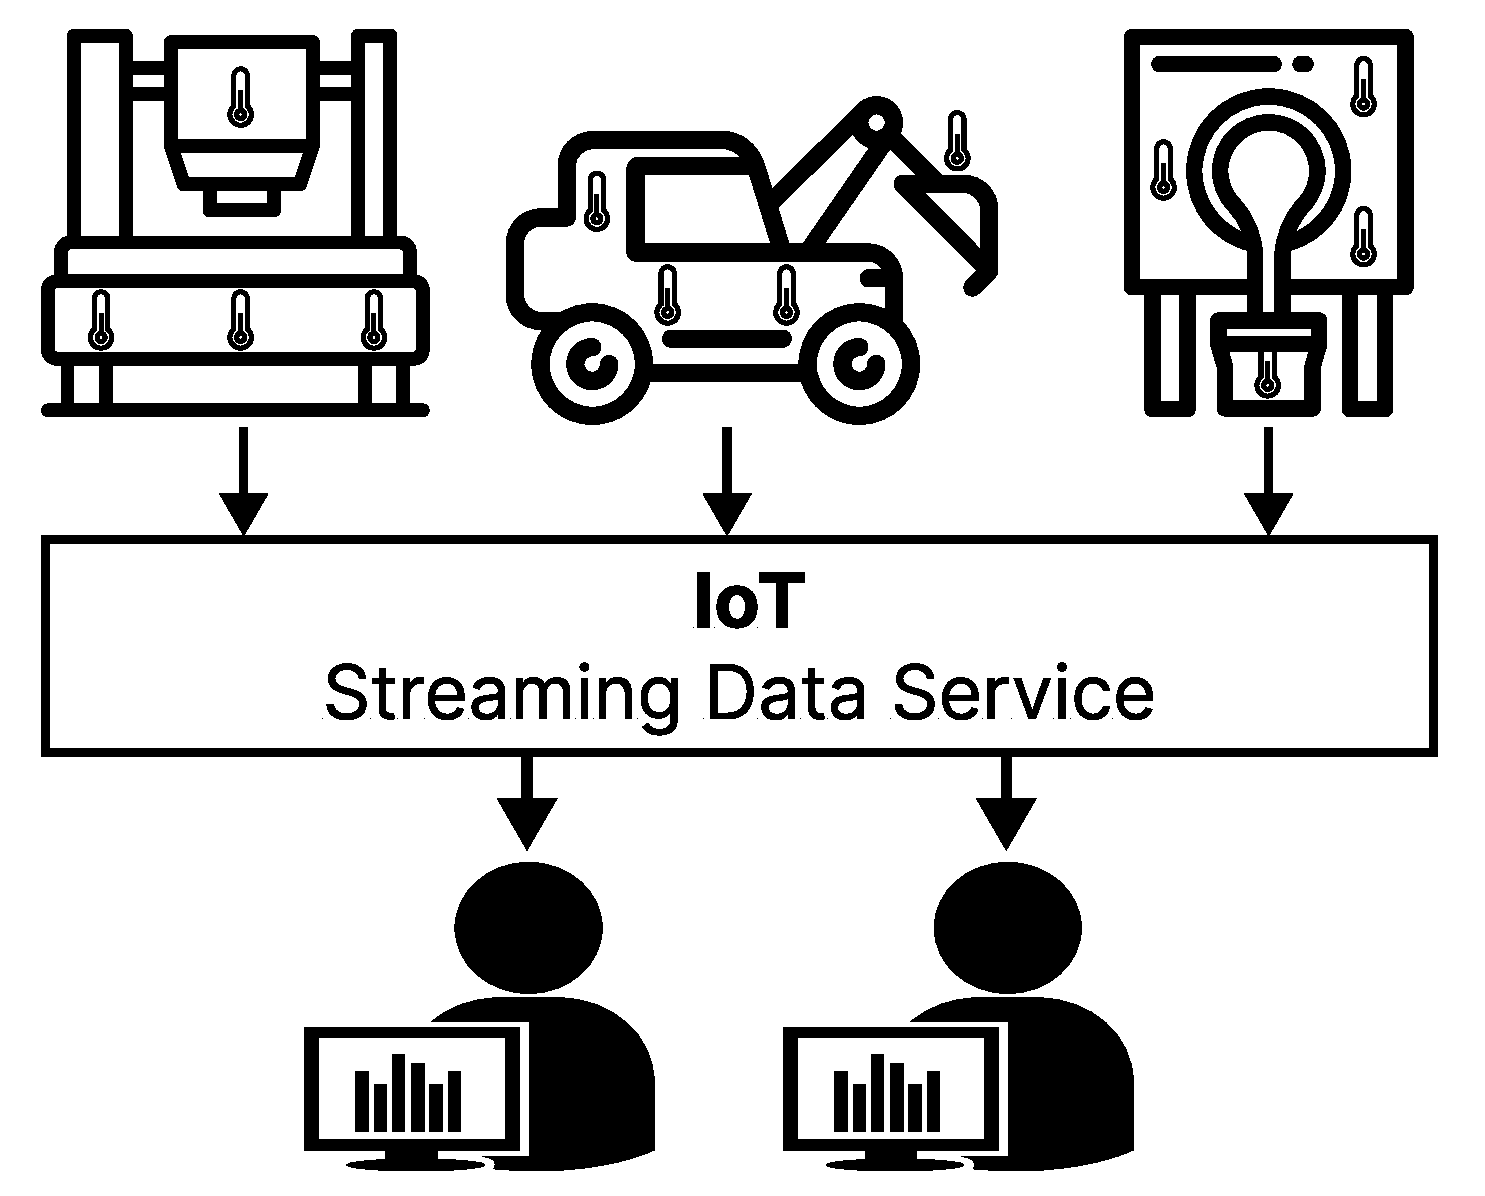
\includegraphics[width=\linewidth]{iot_example_schematic.pdf}
\caption{Schematic of the IoT streaming data service example}
\label{fig:iot_example}
\end{figure}

For example, consider a simple IoT streaming data service that monitors temperature sensors on large pieces of machinery as visualized in Figure~\ref{fig:iot_example}. Each machine is equipped with dozens of sensors that collect a temperature reading every second. Users monitor the machines by querying for temperature aggregates at different levels of granularity.

The input data for our data service consists of sensor information and sensor readings. The data maps onto the following table structure\footnote{We are using a pseudo-SQL syntax for the examples in this paper and assume basic familiarity with SQL. We recommend~\cite{} as an introduction to SQL.}:
\begin{lstlisting}[language=SQL]
CREATE TABLE Sensors (
    sensorid int,
    machineid int
);

CREATE TABLE SensorReading (
    sensorid int,
    time timestamp,
    temperature decimal
);
\end{lstlisting}

To get a broad overview, users look at one hour temperature averages over the last week. To analyze a machine's recent performance they observe one minute averages over the last hour. In both cases, we use the median temperature over the last minute for each sensor to smooth the data and remove outliers.

We can express these data transformations and aggregates as a set of 3 views over the input data\footnote{In the view definitions, \emph{avg} and \emph{max} are aggregate functions whereas \emph{minute} and \emph{hours} are time windowing functions that round a timestamp to the previous minute and hour, respectively.}:

\begin{lstlisting}[language=SQL]
CREATE VIEW SensorSmoothReading AS
SELECT sensorid,
    minute(time) as time_min,
    median(temperature) as temp
FROM SensorReading
GROUP BY sensorid, time_min
\end{lstlisting}

\begin{lstlisting}[language=SQL]
CREATE VIEW MachineHourReading AS
SELECT machineid,
    hour(time_min) as time_hour
    avg(temp) as avg_temp
    max(temp) as max_temp
FROM Sensors s
    JOIN SensorSmoothReading r
    ON r.sensorid = s.sensorid
GROUP BY machineid, time_hour
\end{lstlisting}

\begin{lstlisting}[language=SQL]
CREATE VIEW MachineMinuteReading AS
SELECT machineid, time_min
    avg(temp) as avg_temp
    max(temp) as max_temp
FROM Sensors s
    JOIN SensorSmoothReading r
    ON r.sensorid = s.sensorid
GROUP BY machineid, time_min
WHERE time_min + 1 HOUR >= now()
\end{lstlisting}

\emph{"View"} is a database term \ref{} for a table that is defined as a query over other tables and views. A view is a derived table that transforms table data into useful result sets by joining, aggregating, and analyzing rows from existing tables. Those may be intermediate result sets, like the \emph{SensorSmoothReading} view or views that are ultimately queried by end users and applications like the \emph{MachineHourReading} and \emph{MachineMinuteReading} views.

The user queries for our streaming data service can be expressed as the following query templates against the views defined above:

\begin{lstlisting}[language=SQL]
SELECT * FROM MachineHourReading
WHERE machineid = ?
    AND time_hour + 1 WEEK >= now()
\end{lstlisting}
\begin{lstlisting}[language=SQL]
SELECT * FROM MachineMinuteReading
WHERE machineid = ?
\end{lstlisting}

In both cases, we use the question mark to indicate a query parameter that is set by the user or application at runtime. In the queries above, the question mark represents the machine id of a particular machine a user wants to monitor.

In general, a streaming data service can be defined by a set of complex views over external sources of data\footnote{Some of the sources may be static or infrequently changing data. However, to be considered a \emph{streaming} data service, at least one source of data must be a data stream or update frequently (i.e. have a change stream)} and an associated set of query templates.

In Section~\ref{sec:viewstore} we show that existing database technologies cannot efficiently implement such view sets with low latency and high throughput. We propose \emph{View Store} as a category of database systems that determine and execute optimal partial view materialization to support streaming data service use cases with low latency, high throughput querying on predefined views. Section \ref{sec:datasqrl} outlines the implementation of a view store called \emph{DataSQRL} and introduces the unique challenges of view store implementations.

SQL lacks some features needed to implement streaming data services. For our IoT example, we want to implement automatic alerts when machine temperatures exceed a certain threshold. SQL does not support "reacting" to changes in data. We propose an extension of SQL called \emph{SQRL} - for \emph{Structured Query and \textbf{Reaction} language} - in Section \ref{sec:sqrl} that adds the concept of \emph{subscriptions} for observing and reacting to changes in data. SQRL adds some additional convenience features to SQL that improve developer productivity for implementing streaming data services without changing the semantics of the relational algebra that SQL is based on.

We conclude this paper with a review of common streaming data service use cases, their implementation in SQRL, and compare the performance of DataSQRL to popular relational database systems like Postgres, MySQL as well as special-purpose databases like Neo4j and Timescale in Section \ref{sec:experiments}. Our experiments show that DataSQRL outperforms existing database engines by a factor of x-y. More significant, but also harder to measure, are the improvements in productivity that developers gain by using DataSQRL for their streaming data service implementations.

\section{Implementing Streaming Data Services}
\label{sec:viewstore}

In this section we review current approaches to implementing streaming data services using our IoT example and demonstrate the need for a new type of database system, called \emph{View store}, that support partial maintenance of complex views over streams of data.

A straight-forward way to implement the IoT example would be to write the sensor readings into a database table, install the views defined above, and execute the application queries against those views. We are going to outline how such implementations would perform in practice on various types of database systems.

\subsection{Transactional Database}

A transactional (i.e. row-oriented) database like Postgres \ref{}, MySQL \ref{}, SQLServer \ref{}, or Oracle \ref{} would be able to quickly ingest the streaming sensor data. However, executing the first query asking for a week of average machine temperatures would require retrieving and aggregating over 6 million records for a machine with 10 sensors. Even with carefully tuned index structures and compaction strategies, the data would likely be scattered over multiple non-consecutive disk pages which leads to lengthy data fetch operations that exceed our latency requirements. To reliably achieve responsive query answers within 100 milliseconds\footnote{100 milliseconds is widely considered the threshold for responsive user interactions.} the data would need to be held in memory. However, that is very expensive for the amount of data we are dealing with. Assuming we are monitoring 10000 machines with an average of 20 sensors each, we ingest half a trillion records a month. And even with powerful hardware that has this much RAM, the tail query latencies for machines with 100s of sensors would likely still exceed the 100 millisecond latency threshold when the workload is high (i.e. many users are concurrently monitoring machines).

\subsection{Data Warehouse}

A data warehouse (i.e. column-oriented) database like BigQuery \ref{}, Snowflake \ref{}, Redshift \ref{}, or Vertica \ref{} would reduce the cost of storing the data because of greater storage efficiency, usage of cheaper secondary storage modes, and absence of index structures. However, a data warehouse would not be able to achieve low latency response times to our queries. A data warehouse is optimized for queries that scan a large percentage of the entire stored data. While 6 million records is a substantial amount of data, it is a tiny fraction of the total data stored which makes column scans inefficient. Assuming we are monitoring 10000 machines, our queries would filter out all but 0.01\% of data. Even on powerful hardware, a data warehouse would be unable to achieve low latency response times when the workload is high because of the cost of those expensive scans.

\subsection{Analytics Engine}

The downside to using either type of database system is that we are storing a lot of data that the user isn't directly querying for which is costly in terms of data storage and the computation needed at query time. An analytics engine like Apache Spark \ref{} or Hadoop \ref{} is able to precompute the \emph{MachineHourReading} and \emph{MachineMinuteReading} views in batch and store only the resulting rows in a database for query answering. That greatly reduces the amount of data stored in the database and the computation needed to return the user query results. However, the downside of using an analytics engine in combination with a database is the long latency until new sensor readings can be queried. If we re-compute the views every hour, we have to wait up to 60 minutes before sensor readings can be queried. That's not acceptable since users may not be able to spot issues with the temperature before it is too late. Recomputing views very often is expensive since we have to read the entire data and compute all the aggregates before writing them into the database. And even if we use a lot of hardware, it will likely still takes minutes for the entire batch computation process and database update to complete.

\subsection{State of the Art}

Using existing data systems to implement streaming data service is either too expensive or does not meet latency requirements. Our simple IoT use case demonstrates that (in-memory) databases are too expensive for the data volume and have high tail query latencies, data warehouses do not meet our query latency requirements, and analytics engines do not meet our data latency requirements.

To implement streaming data services in practice, developers have to build custom architectures that combine multiple data systems to achieve the latency requirements at reasonable cost.

A popular approach is the lambda architecture \ref{} which combines the periodic batch computation of the analytics engine with a feed that writes recent data directly into the database. At query time, the data from the batch computed view is combined with the recent data to provide an up-to-date view.

Another approach is to build a data pipeline with custom scripts that build incrementally maintained materialized views which are stored in a database for querying.

Custom architectures are complex, expensive to implement and maintain, and hard to reason about. For every streaming data service use case, developers have to build a custom, hand-tuned database engine from multiple components that need to be orchestrated. Building such architectures that work reliably in practice, accommodate edge cases, and can be holistically monitored requires an extraordinary amount of work and expertise.

The high cost and lack of developer expertise result in implementation failures and lack of adoption of streaming data services despite the benefits they provide to data-driven applications.

\subsection{View Store}
\label{sec:viewstoredef}

We propose \emph{View Store} as a type of database system that meets the requirements of streaming data services and fills the gap in the current database landscape.

A view store is a database system that supports low latency, high throughput querying on a set of pre-defined views over multiple external sources of streaming data.

Let's look at the 3 elements that define a view store in more detail.

To meet the requirements of streaming data services, a view store has to provide low query and data latencies with high query and data throughput.
The time it takes to process new data is called the \emph{data latency} which measures the time from new data being available until all updates triggered by that data have been processed and the results are accessible. The time it takes to answer an application request is called the \emph{query latency} which measures the time that it takes to answer a request for data and return the result. Data latency requirements for streaming data services are usually on the order of seconds whereas query latency requirements are on the order of 100 milliseconds\footnote{Required latency times differ between use cases. The numbers provided here are best practice requirements across a number of use cases}.
The number of new data records that need to be ingested and processed across all data sources per time interval is called the \emph{data throughput}. The number of user or application requests that must be answered per time interval is called the \emph{query throughput}.

A view store requires that the set of views and query templates accessed by the application are registered up front. That's the biggest difference to traditional database systems\footnote{Most databases treat views as registered queries and allow for arbitrary queries at runtime} and the key to meeting the throughput requirements. The views and query templates of a streaming data service are determined by the calling application, which means they are static when the application is deployed and only evolve during development cycles. Knowing the views, structure of the queries, and sources of data over which those are defined up front allows a view store to determine the optimal materialization strategy. Whereas traditional database systems find the fastest query plans against pre-defined data and index structures, a view store determines the optimal tradeoff between (partial) view materialization and query plans against the materialized views to meet latency requirements at low cost. We discuss optimization in more detail in Section~\ref{sec:optimization}.

Lastly, view stores consume data from one or multiple sources of streaming and static data. Most database systems assume that the data is explicitly inserted into pre-defined data structures. Federated database systems support multiple sources of data but do not support low query latencies for complex views since they need to fetch the data from the source systems at query time. View stores consume external data but build their own internal data structures to provide fast query access.

View stores are a specialized type of database system that meet the requirements of streaming data services. As streaming data services become more prevalent, we need view stores as a dedicated database category to support their implementation.
In Section~\ref{sec:datasqrl} we outline the implementation of the DataSQRL view store and provide more details on how view stores differ from other types of databases.

\section{SQRL}
\label{sec:sqrl}

SQRL, which stands for "Structured Query and Reaction Language", is an extension to the database query language SQL that accommodates the following needs of streaming data service implementations: 1) being able to "react" to changes in data and converting data streams to stateful data, 2) increasing developer productivity for defining sets of complex views, 3) explicitly defining relationships and local scopes, 4) natively handling hierarchical data, and 5) providing flexible, programmatic query access via API.

The motivation for SQRL is twofold. First, SQRL adds features to SQL needed for handling streaming data - in particular, reacting to changes in data and hence the "R" in "SQRL".
Second, SQRL adds a number of developer productivity and convenience features to make the language more appealing to software developers of streaming data services.

SQRL does not change the semantics of SQL and is based on the same relational algebra. SQRL can be translated to SQL as described in Appendix~\ref{appendix:sqrl2sql}, but the resulting syntax tends to be much more verbose and harder to understand.

\subsection{Reacting to Data Changes: State vs Events}

A streaming data service often needs to react to changes in the data to trigger actions.
For our IoT example, we want to be alerted when the maximum temperature on a machine exceeds $100^{\circ}$ Celsius.

SQRL supports \emph{subscriptions} which create an event record whenever a particular change event is observed on an underlying view.

\begin{lstlisting}[language=SQL]
CREATE SUBSCRIPTION HighTemp
ON ADD AS
SELECT machineid, time_min, max_temp
FROM MachineMinuteReading
WHERE max_temp > 100
\end{lstlisting}

This example defines the \emph{HighTemp} subscription which creates an event record with \emph{machineid}, \emph{time\_min}, and \emph{max\_temp} whenever a max temperature reading in the \emph{MachineMinuteReading} view is greater than 100. We call the view definition (i.e. the part after "AS") the \emph{observed view}.

A subscription specifies which type of change against the observed view triggers an event:
\begin{enumerate}
    \item \textbf{ON ADD}: Creates an event record whenever a row is newly added to the observed view.
    \item \textbf{ON CHANGE}: Creates an event record whenever a row in the observed view changes
    \item \textbf{ON DELETE}: Creates an event records whenever a row is removed from the observed view.
\end{enumerate}

Subscriptions define additional tables in the logical model that contain rows for each observed event. Subscriptions create event streams from stateful data based on user defined criteria. That means we can build on subscriptions, export them to downstream consumers, and treat them like any other data stream.

When building streaming data services, we distinguish between \emph{streaming} and \emph{stateful} data. Both types of data are represented as rows with column structure but the way we interact and use the data depends on the type.

The \emph{SensorReading} input table contains streaming data. Every second that a sensor produces a temperature reading, an event record is created that is added to the table. Streaming data represents events that happen at a point in time and streaming data records usually have a timestamp column to mark that time.

The \emph{Sensors} input table contains stateful data. Every row captures the state of a sensor entity, i.e. it's placement on a particular machine. Stateful data represents the state of an entity. Stateful data has a natural key (i.e. a subset of columns) which uniquely identifies the entity that the state is assigned to. For \emph{Sensors} the natural key is the \emph{sensorid} column. We expect there to only be a single row for each sensorid since a sensor can only be placed on one machine at a time. In contrast, we make no such uniqueness assumptions for streaming data.

SQRL treats all input data as sources of streaming to avoid making assumptions about the data. The user determines what type of data each table represents by how the data is used. In our IoT example we are joining directly against the \emph{Sensors} table in computing the machine temperature aggregates which implies that the data is stateful, such as coming from a file that contains the unique sensor to machine mappings.

We would have to treat the \emph{Sensors} table differently if it was streaming data, such as a change stream from a database system that keeps track of what machine a particular sensor is placed on. In that case, \emph{sensorid} is no longer a natural key because the data represents changes in sensor placement over time and the same $sensorid$ occurs multiple times when a sensor changes placement. To determine our temperature aggregates, we would only be interested in a sensors most recent location.

SQRL provides the \emph{DISTINCT ON} statement to convert such change streams into stateful data.
\begin{lstlisting}[language=SQL]
CREATE VIEW Sensors AS
DISTINCT Sensors ON sensorid
    ORDER BY _ingest_time DESC;
\end{lstlisting}
This definition redefines the \emph{Sensors} table as a stateful view by taking the most recent change event for each \emph{sensorid}. The \emph{\_ingest\_time} column is automatically added to input table rows and captures the time at which the record was ingested into the system. For streaming data sources that don't have a timestamp column the \_ingest\_time column provides a useful alternative.

More generally, the \emph{DISTINCT ON} statement converts a data stream of changes into stateful data by taking the first row according to the specified order for each unique value of the natural key columns specified after \emph{ON}.

We can also use standard SQL statements to convert streaming to stateful data. The \emph{MachineHourReading} and \emph{MachineMinuteReading} view definitions use \emph{GROUP BY} to aggregate the streaming \emph{SensorSmoothReading} data into time buckets for each machine as stateful data with the \emph{machineid} and time bucket columns as natural key.

In addition to aggregating over time windows, SQRL also makes it easy to define "most recent" aggregates. To track the highest temperature reading per machine over the last 24 hours, we can define the following view:
\begin{lstlisting}[language=SQL]
CREATE VIEW MachineRecentMaxTemp AS
SELECT machineid,
    max(temp) as max_temp
FROM Sensors s
    JOIN SensorSmoothReading r
    ON r.sensorid = s.sensorid
WHERE time_min + 24 HOUR >= now()
GROUP BY machineid
\end{lstlisting}

This defines a maximum temperature aggregate for each machine over a sliding window of time that extends over the last 24 hours. SQRL provides the special \emph{now()} function which stands for the current time as a convenient way to define sliding time windows and filter records by recency.

Finally, we can also use the familiar \emph{SELECT DISTINCT} statement to convert data stream to stateful data by deduplicating a data stream into unique data tuples. For example, we define a stateful view that contains all the machines we are monitoring as follows:
\begin{lstlisting}[language=SQL]
CREATE VIEW Machines AS
SELECT DISTINCT machineid
FROM Sensors
\end{lstlisting}

When building streaming data services it is important to distinguish between streaming and stateful data. SQRL extends SQL by features that make it easy to seamlessly convert between the two. \emph{DISTINCT ON} and time-window aggregates using \emph{now()} and time window functions produce stateful data from data streams in addition to the standard SQL aggregation based on \emph{SELECT DISTINCT}. Subscriptions go the other way and produce event streams from stateful data.


\subsection{Developer Productivity}

SQL is a great language for defining queries over tabular data. For software development, developers prefer languages that are easy to read for larger bodies of code, convenient to use, and allow for incremental development. SQRL adds languages features to SQL to make it more developer friendly.

Developers implement streaming data services in SQRL scripts. An SQRL script first declares the (streaming) data sources that it builds on using \emph{IMPORT} statements. Our IoT example has the following imports:
\begin{lstlisting}[language=SQL]
IMPORT sensordata.SensorReading
IMPORT sensordata.Sensors
\end{lstlisting}

An import statement has two parts: the name of the data source and the name of the table to import from that source. Data sources can be queues, file systems, logs, etc and are configured under a unique name. We discuss data sources in more detail in Section~\ref{sec:datasqrl-source}.
We can also import all tables from a data source via \emph{IMPORT sensordata.*}. Once imported, the tables can be referenced in \emph{FROM} clauses of view definitions.

To reduce the verbosity of the SQL view definition syntax, SQRL adds the assignment operator $:=$ as a syntactic shorthand for definitions.

\begin{lstlisting}[language=SQL]
SensorSmoothReading := SELECT sensorid,
    minute(time) as time_min,
    median(temperature) as temp
FROM SensorReading
GROUP BY sensorid, time_min
\end{lstlisting}

SQRL supports incremental view definitions and redefining existing views and columns. This is particularly useful for data cleansing and data normalization which are frequently part of streaming data service implementations.

For example, most of our sensors produces readings with a \emph{temperature} column that contains the Celsius value. However, some older sensors produce a reading with a \emph{temperature\_f} column in Fahrenheit. To normalize the data, we redefine the \emph{temperature} column on the \emph{SensorReading} table as follows.

\begin{lstlisting}[language=SQL]
SensorReading.temperature :=
    coalesce(temperature,
        (temperature_f - 32)/9*5)
\end{lstlisting}

This statement overrides the \emph{temperature} column so that any subsequent references to that column table resolve to the correct temperature.

SQRL scripts can import views defined by other scripts in order to facilitate reuse of data transformations and analytics between data services. To share our definition of \emph{SensorSmoothReading} between scripts, we can place it in a script called \emph{sensorshared} and then import the view:
\begin{lstlisting}[language=SQL]
IMPORT sensorshared.SensorSmoothReading
\end{lstlisting}

All public views and columns are accessible by the importing script. Views and columns with names starting with an underscore are private and not accessible outside the script.

To connect subscription data streams to outside consumers, SQRL supports \emph{EXPORT} statements.
\begin{lstlisting}[language=SQL]
EXPORT HighTemp TO alerts.TempAlert
\end{lstlisting}
Assuming we have a data sink with the name \emph{alerts} registered, this statement exports all event records created by the subscription into the data sink under the \emph{TempAlert} namespace.

\subsection{Relationships and Local Scopes}

SQRL adds the concept of \emph{relationships} to SQL in order to improve code readability, simplify the conceptual model, and make it easier to handle hierarchical data.

A column can be defined as a relationship column using a JOIN clause to relate rows from one table or view to those from another.
\begin{lstlisting}[language=SQL]
Sensors.readings :=
JOIN SensorSmoothReading r
    ON r.sensorid = _.sensorid
\end{lstlisting}

This statement defines a relationship column \emph{readings} on the table \emph{Sensors} as a natural join with \emph{SensorSmoothReading}.
The underscore in the join condition is the alias for the view on the left-hand side of the assignment operator, i.e. \emph{Sensors}, that's automatically assigned by SQRL.

Relationship columns represent a logical join that gets instantiated when the column is accessed in a view definition or column expression. For example, we can simplify the join clause of the \emph{MachineRecentMaxTemp} view using the relationship column:
\begin{lstlisting}[language=SQL]
CREATE VIEW MachineRecentMaxTemp AS
SELECT machineid,
    max(temp) as max_temp
FROM Sensors s JOIN s.readings r
WHERE time_min + 24 HOUR >= now()
GROUP BY machineid
\end{lstlisting}

The join with \emph{s.readings} expands to the full join declaration from above with the table alias $s$ filling in for the underscore alias placeholder, which means the above view definition is equivalent to the original one.

Relationship columns allow us to reuse join declarations across view definitions and column expressions as well as label a relationship explicitly to support code readability.

Another feature that SQRL introduces is the concept of localized scopes to break out sub-queries and define them incrementally. To track the number of sensors that are placed on each machine, we could update the \emph{Machines} view and add a column:

\begin{lstlisting}[language=SQL]
CREATE VIEW Machines AS
SELECT machineid,
(SELECT count(*) FROM
Sensors s WHERE
s.machineid = m.machineid)
    AS sensorcount
FROM
(SELECT DISTINCT machineid
FROM Sensors) m
\end{lstlisting}

View definitions with nested sub-queries are hard to read. In SQRL we can break out the $sensorcount$ sub-query and implement it as an incremental column definition:
\begin{lstlisting}[language=SQL]
Machines.sensorcount :=
SELECT count(*) FROM
Sensors s WHERE
s.machineid = _.machineid
\end{lstlisting}

This statement adds the $sensorcount$ column to the previously defined $Machines$ view. The underscore refers to the $Machines$ view on the left-hand side of the assignment and defines this query in localized scope, i.e. as a nested sub-query.

Localized scope is particularly useful in combination with relationships. Instead of defining the entirely separate view \emph{MachineRecentMaxTemp} to capture the maximum recent temperature of a machine, we can do so by adding another relationship and column to \emph{Machines}:

\begin{lstlisting}[language=SQL]
Machines.sensors := JOIN Sensors s
    ON s.machineid = _.machineid

Machines.maxRecentTemp :=
SELECT max(temp) FROM _.sensors.readings
WHERE time_min + 24 HOUR >= now()
\end{lstlisting}

$sensors$ defines a relationship column that relates rows in $Machines$ to the $Sensors$ that are placed on them through a natural join. The $maxRecentTemp$ column is a localized sub-query that aggregates the maximum temperature for all sensors readings per machine. The expression $\_.sensors.readings$ is a concatenated relationshiop expression that combines the join declarations from the two relationships.
The complete view definition in SQL is shown in Figure~\ref{fig:machinesView} and demonstrates the convenience and utility of SQRL sytnax.

\begin{figure*}
\begin{lstlisting}[language=SQL]
CREATE VIEW Machines AS SELECT machineid,
   (SELECT count(*) FROM Sensors s
    WHERE s.machineid = m.machineid) AS sensorcount
   (SELECT max(temp) FROM Sensors s
    JOIN SensorSmoothReading r ON r.sensorid = s.sensorid
    WHERE s.machineid = m.machineid AND
          time_min + 24 HOUR >= now()) AS maxRecentTemp
FROM (SELECT DISTINCT machineid FROM Sensors) m
\end{lstlisting}
\caption{Example of how SQRL syntax expends to standard SQL}
\label{fig:machinesView}
\end{figure*}

To compute the current temperature of each machine as the average of the most recent temperature reading for all sensors on the machine, we define a $lastReading$ relationship on sensors that relates a sensors to it's most recent temperature reading:

\begin{lstlisting}[language=SQL]
Sensors.lastReading :=
JOIN SensorSmoothReading r
    ON r.sensorid = _.sensorid
    ORDER BY r.time_min DESC LIMIT 1
\end{lstlisting}

Adding a \emph{LIMIT} to the join clause of a relationship definition constrains the multiplicity of the relationship. The \emph{ORDER BY} clause determines which related records are part of the relationship. We use the $lastReading$ relationship to compute the temperature average as follows:

\begin{lstlisting}[language=SQL]
Machine.currentTemp := SELECT avg(temp)
    FROM _.sensors.lastReading
\end{lstlisting}

Expressing a multiplicity restricted join in SQL is cumbersome and requires a nested \emph{PARTITION OVER} query that assigns a row number to filter on. Figure~\ref{fig:machinesPartitionOver} shows the equivalent SQL syntax.

\begin{figure*}
\begin{lstlisting}[language=SQL]
CREATE VIEW Machines AS SELECT machineid,
   ...
   (SELECT avg(temp) FROM Sensors s JOIN
     (SELECT sensorid, temp FROM
        (SELECT sensorid, temp,
        row_number() OVER (PARTITION BY sensorid ORDER BY time_min DESC)
            AS row_no
        FROM SensorSmoothReading)
     WHERE row_no = 1) r ON r.sensorid = s.sensorid
   WHERE s.machineid = m.machineid) AS currentTemp
FROM (SELECT DISTINCT machineid FROM Sensors) m
\end{lstlisting}
\caption{Example of how SQRL syntax expends to standard SQL}
\label{fig:machinesPartitionOver}
\end{figure*}

When aggregating a single column over a to-many relationship, SQRL supports a convenience syntax to specify the relationship path inside the aggregate function. This allows us to simplify the $currentTemp$ column definition to:

\begin{lstlisting}[language=SQL]
Machine.currentTemp :=
  avg(sensors.lastReading.temp)
\end{lstlisting}

\subsection{Representing Hierarchical Data}

Many data services need to consume hierarchically structured data such as JSON documents. SQRL natively supports hierarchical data through nested tables with parent-child relationships to eliminate the cumbersome work of mapping between hierarchical and relational data.

For example, our IoT application allows users to define \emph{monitoring groups} to monitor groups of machines, such as a fleet of vehicles or all machines on a factory floor. Monitoring Groups are stored as JSON objects like the following:

\begin{lstlisting}
{
  groupid: 501,
  groupName: "Wenatchee Factory",
  machines: [
   {
     machineid: 1075,
     machineName: "Mill Saw"
   },
   {
     machineid: 1098,
     machineName: "Wood Grinder"
   }
  ]
}
\end{lstlisting}

In SQRL, this data can be imported like any other table via
\begin{lstlisting}
IMPORT iotapp.MonitorGroup
\end{lstlisting}

Internally, SQRL creates two tables: \emph{MonitorGroup} with columns $groupid$, $groupName$, and a relationship column $machines$ that relates to the respective rows in the nested table \emph{MonitorGroup.machines} which has the columns $machineid$, $machineName$, and a relationship column $parent$ which relates it back to the parent table row. SQRL creates a hidden primary key for the nested table that combines the primary key of the parent table with the local primary key of the nested table, e.g. the index offset in the array for our example data. The primary key of a table is either the natural key if one exists or the $\_uid$ column which is added by SQRL to contain a unique identifier for each row.

SQRL maps nested data onto separate tables related by shared primary key and uses relationship columns to explicitly relate the tables in the logical model to allow the user to navigate the hierarchical structure.

For example, we can compute the number of machines in a monitoring group by counting the relationship column:
\begin{lstlisting}[language=SQL]
MonitorGroup.numMachines :=
                count(machines)
\end{lstlisting}

Nested tables can be treated and extended like any other table with the only difference that nested table names are paths. For example, we can add a relationship column that relates the machines in a monitoring group to the \emph{Machines} view:
\begin{lstlisting}[language=SQL]
MonitorGroup.machines.machine :=
  JOIN Machines m
  ON m.machineid = _.machineid
\end{lstlisting}

SQRL automatically defines nested tables in the data model when the input data is hierarchically structured. In addition, the user can defined nested tables explicitly to group by the parent table.

For example, the following nested table computes the temperature maximums and averages by 1 hour time window for all the machines in a monitoring group:
\begin{lstlisting}[language=SQL]
MonitorGroup.hourReading :=
SELECT hour(time_min) as time_hour,
       avg(temp) as avg_temp,
       max(temp) as max_temp
FROM _.machines.machine.sensors.readings
GROUP BY time_hour
\end{lstlisting}

Because this query defines a nested table under the \emph{MonitorGroup} table, the grouping by parent table primary key is implied which simplifies the syntax.

Relationship columns, localized query statements, and nested tables support an object-oriented thinking that many developers are familiar with and simplifies query statements. By making relationships in the data explicit, developers can directly translate their conceptual entity-relationship model into SQRL without intermediate translation.

All of these features extend the syntax of SQL but not the semantics of the underlying relational algebra. Appendix~\ref{appendix:sqrl2sql} details how SQRL translates to SQL.

\subsection{Programmatic Query Access via API}

Streaming data services are often accessed programmatically through an API from an application or developer code. SQRL automatically generates an API from the views and relationships that are defined in an SQRL script to reduce the boilerplate code developers have to write and narrow the impedence mismatch between the relational model and the object-oriented model of many development languages.

SQRL generates GraphQL and REST APIs where each table and view defined in the SQRL script gets exposed as an entity and each relationship is exposed as a traversable reference.

For our IoT data service, the generated API supports the following GraphQL query to retrieve information about and the last 24 hours of aggregating sensors readings for a monitoring group:

\begin{lstlisting}
monitoringGroup(filter =
            {groupid: {eq: 501}}) {
    groupName
    machines {
        machineId
        machineName
    }
    hourReading (limit: 24,
      order: [{time_hour: DESC}]) {
        time_hour
        avg_temp
        max_temp
    }
}
\end{lstlisting}

Each public view and table is exposed as a type of the same name in the GraphQL schema and a query endpoint. $monitoringGroup$ in the query above is the query endpoint for the $MonitoringGroup$ view in the SQRL script. The query endpoints return the type of the same name which has a field for every public column of the view/table that it represents.
The filter attribute on the query endpoints allow users of the API to filter the rows returned by the endpoint. The example above uses the filter to return the monitoring group with id equal to $501$. The filter attribute allows API users to construct $WHERE$ clauses by logical conjunction of predicates on the columns defined in the view.

In addition, users can specify an order and limit to control the returned results. Relationships can be traversed through the GraphQL API as references and offer the same filter, order, and limit attributes as query endpoints. The example traverses through the $hourReading$ relationship to the nested table that contains the temperature aggregates. The $order$ and $limit$ attributes restrict the result set to the last 24 hours of readings. A more formal definition of the GraphQL and REST API generation is provided in Appendix~\ref{appendix:sqrl2graphql}.

The generated GraphQL API allows developers to build nested \emph{SELECT} clauses over the views and tables defined in the SQRL script by traversing through relationships and specifying the columns to return. Developers can restrict the result set by applying filters, i.e. conjunctive \emph{WHERE} clauses, orders, and limits. Thereby, GraphQL queries map onto SQL queries against the defined views and tables. The API provides full programmatic access to the data transformations defined in the SQRL script. Unlike ORM layers and libraries, there is a direct mapping between the API and the underlying data which means there is no need to break out into SQL to get "full" query access.

\subsection{Complete Example}

\begin{lstlisting}[language=SQL]
IMPORT sensordata.*;
IMPORT iotapp.MonitorGroup;

Sensors := DISTINCT Sensors ON sensorid
    ORDER BY _ingest_time DESC

SensorReading.temperature :=
    coalesce(temperature,
        (temperature_f - 32)/9*5);

Sensors.readings :=
    SELECT minute(time) as time_min,
        median(temperature) as temp
    FROM SensorReading r
    WHERE r.sensorid = _.sensorid;



Sensors.temps :=



MonitorGroup.hourReading :=
SELECT hour(time_min) as time_hour,
       avg(temp) as avg_temp,
       max(temp) as max_temp
FROM _.machines.machine.sensors.readings
GROUP BY time_hour
\end{lstlisting}


\section{DataSQRL}
\label{sec:datasqrl}

DataSQRL is a view store implementation based on SQRL. The high-level architecture of DataSQRL is shown in Figure~\ref{fig:datasqrl_architecture}. The DataSQRL orchestrator provides an API for developers to compile and deploy SQRL scripts, connect data sources and sinks, and monitor the system.

\begin{figure}[h]
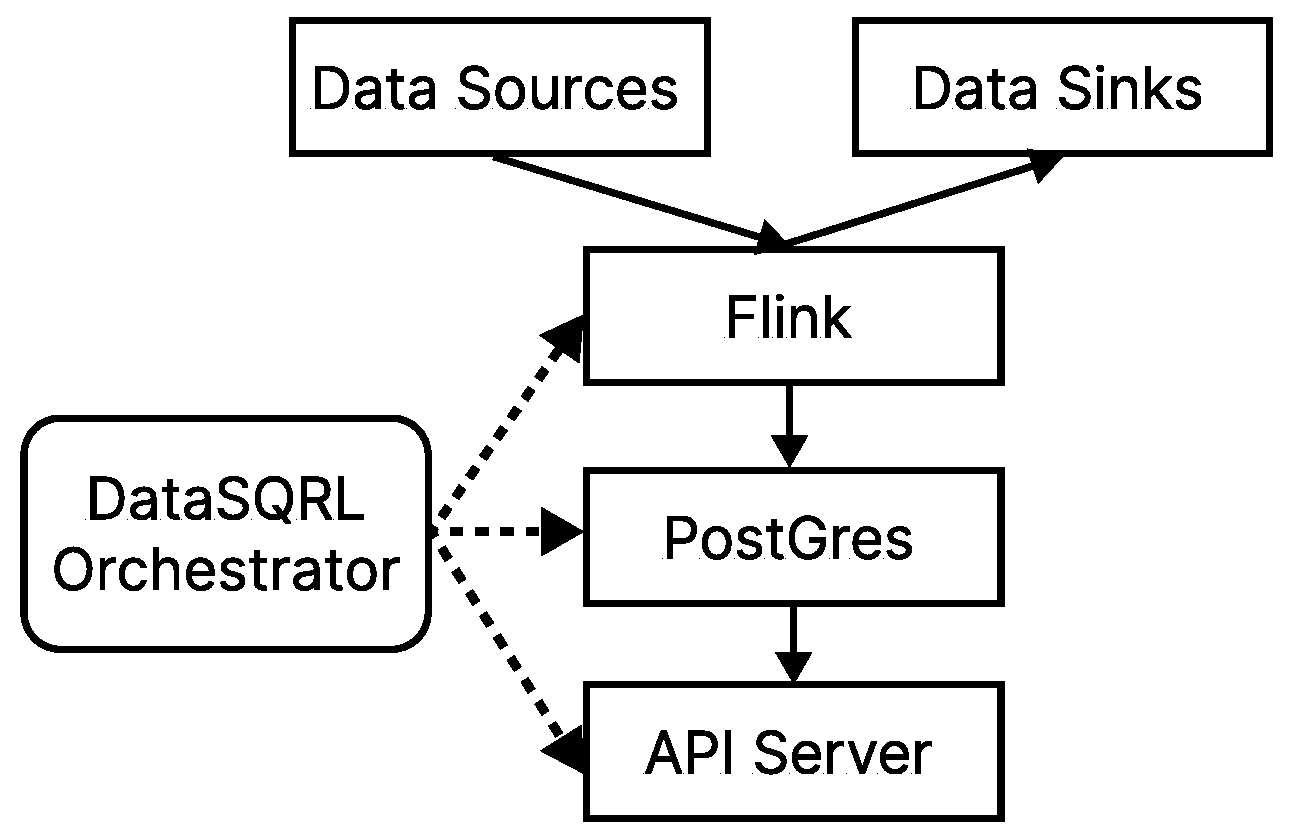
\includegraphics[width=\linewidth]{datasqrl_architecture.pdf}
\caption{High level architecture of DataSQRL}
\label{fig:datasqrl_architecture}
\end{figure}



\subsection{Sources and Sinks}
\label{sec:datasqrl-source}
Data Sources

infering water marks or cofigure them explicitly in import
managing retractions for stragglers within bounded window (configurable)

\subsection{Compilation}
\label{sec:compilation}

\subsection{Optimization}
\label{sec:optimization}


\section{Experiments}
\label{sec:experiments}


\section{Related Work}
\label{sec:related}

The SQRL query language is inspired by the work of Widom et al. on the CQL query language~\cite{arasu_cql_2006} for streaming database systems~\cite{arasu_stream_2016}.

Hasura for automatic API generation

\section{Conclusion}
\label{sec:conclusion}



\appendix

\section{Translating SQRL to SQL}
\label{appendix:sqrl2sql}

We infer watermark timestamp for streaming data sources and only consider closed time buckets when watermark is used in GROUP BY. However, there may be stragglers which causes retractions - even in downstream data sinks using

but detailed description from google doc in here

\section{Generating GraphQL schema from SQRL data model}
\label{appendix:sqrl2graphql}


\section{Scrap Space}

%------------

Streaming data services need to provide low latency response times to both newly incoming data (e.g. a new user action that updates the recommendations for this user) and to user requests (e.g. a user viewing their recommendations in a mobile app). Likewise, streaming data services need to support high throughput for incoming data (e.g. the number of user action records per second) and user requests (e.g. the number of concurrent users viewing their recommendations).

Implementing streaming data services that meet these requirements is very costly, time consuming, and error prone because of the lack of suitable data technologies and a complex developer ecosystem. Because streaming data services are difficult to implement in practice, their adoption has been relatively slow outside of a few technology companies with the talent and resources to build them successfully, despite the fact that the data-driven features and data-intensive applications they facilitate can deliver significant value to an organization.

There is no single data technology that developers can use to implement a streaming data service that meets application requirements. As a consequence, actual implementations combine multiple data technologies like batch-processing, databases, ETL tools, and data warehouse that are orchestrated through fragile data pipelines and integrated with custom scripts. Such architectures require a lot of time and effort to implement and the resulting complexity makes it hard to reason about the system as a whole which causes errors and significant operational overhead.

%----------

The second obstacle to implementing streaming data services is the complexity of the developer ecosystem and poor usability. To build a streaming data service developers need to have expertise in a fragmented set of tools and languages which do not share a conceptual model, lack interoperability, and require low-level tuning. Therefore, teams implementing streaming data services tend to be large, faced with a steep learning curve, spend a lot of time writing so called \textit{"plumbing"} code that maps data between systems or schemas, and have to hand-optimize the resulting data system.

%------------

For other aspects of streaming data services, SQL is too difficult or cumbersome to use, which causes developers to choose other languages and tools. For data extraction, pre-processing, and integration, developers prefer scripting languages like Python or ETL tools. Streaming view materialization is often implemented procedurally in imperative languages like Java or Go. Developers prefer Python or R for data analysis. Queries are executed through object-relational mappers (ORM). And some data processing may be done in the user-facing application in JavaScript, Ruby, or similar web application languages.

Such a fragmented and complex developer ecosystem reduces developer productivity and makes implementing streaming data services more costly. Since developers fill perceived gaps and shortcoming in SQL with imperative languages, they have to invest a significant amount of time into finding efficient implementations for their data transformations and optimize their code by hand. A declarative language like SQL allows developers to focus on the data transformations and letting the optimizer determine the most efficient implementation. Since the choice of data structures, execution plan, and index structures matters greatly to the performance of a streaming data service, this significantly improves developer productivity.


\printbibliography

\end{document}